The manufacturing sector is driven by the need of increased productivity. The need
for efficiency, precision, safety and cost reduction has led to significant push towards
automation. The industrial growth is currently pushed by the Industrial 4.0: a fourth wave
of technological advancements that is connecting sensors, machines, and other
\hyperref[tab:acronyms]{IT} systems. These connected systems, also known as cyberphysical systems, may communicate with one 
another via common Internet-based protocols and use data analysis to self-configure, anticipate 
failure, and react to changes. Industry 4.0 is making it possible to have
flexibility in production by enabling faster and efficient processes. \cite{BAI2020107776,russmann2015industry}

There are nine pillars of technological advancements, namely big data and analytics, autonomous robots, simulation,
horizontal and vertical system integration, the industrial internet of things,
cybersecurity, the cloud, additive manufacturing, augmented reality. \cite{russmann2015industry}


\begin{figure}[h]
    \centering
    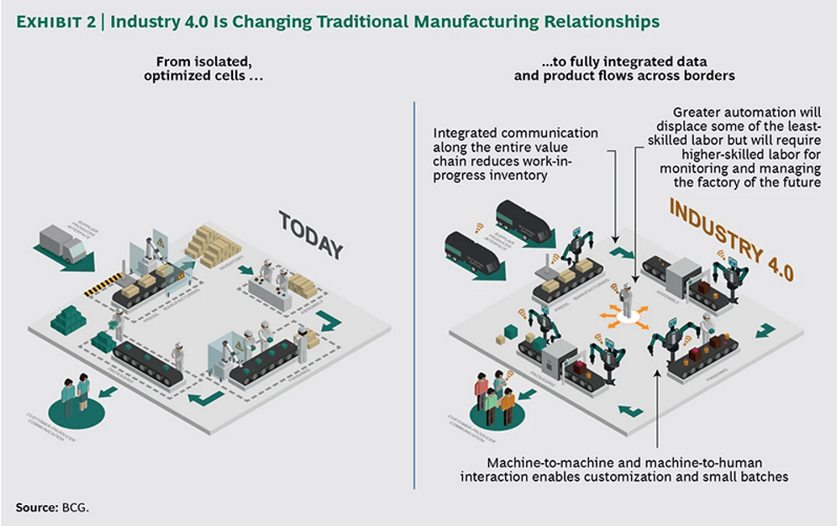
\includegraphics[width=0.75\textwidth]{1. Introduction/1.1 Background/exhibit2.png}
    \caption{Industry 4.0 is changing traditional manufacturing relationships (Source: \cite{russmann2015industry})}
    \label{fig:background-exhibit-2}
\end{figure}

Metal bending processes through an \hyperref[tab:acronyms]{AMADA} bending machine, used to rely heavily upon the
manual labor traditionally. Industry 4.0 is representing a transformation
from low skill manual labor to a sophisticated system that requires \hyperref[tab:acronyms]{IT}-related skills
and innovation abilities in the workforce. Robotic Automation would have less variability in product
quality and will not expose operators to physical strain and repetitive motion injuries. Collaborative robots
with vision sensors \cite{8361333} allows to have flexibility in manufacturing of metal sheets.
It means robot can be programmed to perform bending of different metal sheets when required. \cite{kassowrobotsblog}
